\documentclass[border=10pt]{standalone}
\usepackage{pgfplots}
\usepgfplotslibrary{fillbetween}
\usetikzlibrary{calc}
\pgfplotsset{compat=1.18, trig format plots=deg}
\begin{document}
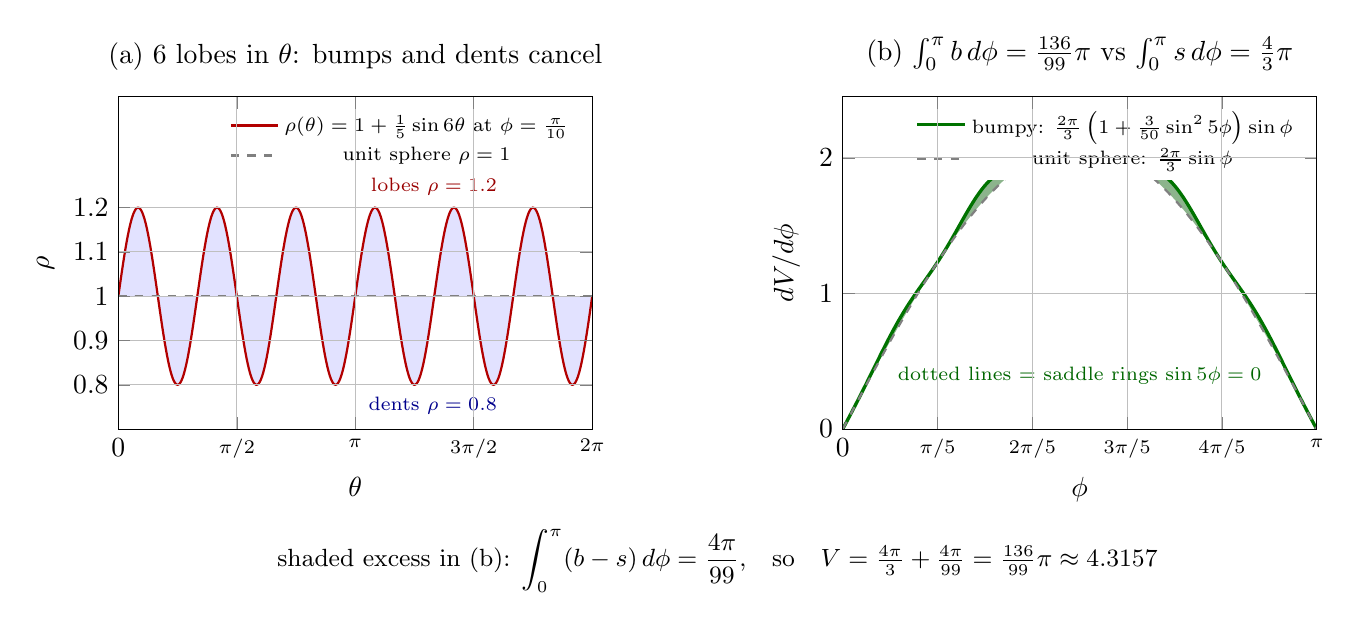
\begin{tikzpicture}
% ---------- panel (a): theta-profile of rho ----------
\begin{axis}[
    name=A, width=7.6cm, height=5.8cm,
    domain=0:360, samples=400,
    xlabel={$\theta$}, ylabel={$\rho$},
    xmin=0, xmax=360, ymin=0.7, ymax=1.45,
    xtick={0,90,180,270,360},
    xticklabels={$0$,${\scriptstyle\pi/2}$,${\scriptstyle\pi}$,${\scriptstyle3\pi/2}$,${\scriptstyle2\pi}$},
    ytick={0.8,0.9,1.0,1.1,1.2},
    grid=major, axis on top,
    title={(a) 6 lobes in $\theta$: bumps and dents cancel},
    legend style={font=\scriptsize, at={(0.98,0.98)}, anchor=north east, draw=none}]
  \addplot[name path=bump, thick, red!70!black] {1+0.2*sin(6*x)};
  \addlegendentry{$\rho(\theta)=1+\frac{1}{5}\sin 6\theta$ at $\phi=\frac{\pi}{10}$}
  \addplot[name path=unit, dashed, gray, thick] {1};
  \addlegendentry{unit sphere $\rho=1$}
  \addplot[blue!25, opacity=0.45] fill between[of=bump and unit];
  \node[font=\scriptsize, red!60!black, anchor=south east] at (axis cs:295,1.205) {lobes $\rho=1.2$};
  \node[font=\scriptsize, blue!55!black, anchor=north east] at (axis cs:295,0.795) {dents $\rho=0.8$};
\end{axis}
% ---------- panel (b): phi-integrand of the volume ----------
\begin{axis}[
    name=B, at={(9.2cm,0)}, width=7.6cm, height=5.8cm,
    domain=0:180, samples=400,
    xlabel={$\phi$}, ylabel={$dV/d\phi$},
    xmin=0, xmax=180, ymin=0, ymax=2.45,
    xtick={0,36,72,108,144,180},
    xticklabels={$0$,${\scriptstyle\pi/5}$,${\scriptstyle2\pi/5}$,${\scriptstyle3\pi/5}$,${\scriptstyle4\pi/5}$,${\scriptstyle\pi}$},
    grid=major, axis on top,
    title={(b) $\int_0^\pi b\,d\phi=\frac{136}{99}\pi$ vs $\int_0^\pi s\,d\phi=\frac{4}{3}\pi$},
    legend style={font=\scriptsize, at={(0.98,0.99)}, anchor=north east, draw=none}]
  \addplot[name path=bb, very thick, green!45!black] {(2*pi/3)*(1+(3/50)*(sin(5*x))^2)*sin(x)};
  \addlegendentry{bumpy: $\frac{2\pi}{3}\left(1+\frac{3}{50}\sin^2 5\phi\right)\sin\phi$}
  \addplot[name path=ss, dashed, gray, thick] {(2*pi/3)*sin(x)};
  \addlegendentry{unit sphere: $\frac{2\pi}{3}\sin\phi$}
  \addplot[green!35!black, opacity=0.45] fill between[of=bb and ss];
  \draw[green!45!black, densely dotted, opacity=0.5] (axis cs:36,0) -- (axis cs:36,1.75);
  \draw[green!45!black, densely dotted, opacity=0.5] (axis cs:72,0) -- (axis cs:72,2.05);
  \draw[green!45!black, densely dotted, opacity=0.5] (axis cs:108,0) -- (axis cs:108,2.05);
  \draw[green!45!black, densely dotted, opacity=0.5] (axis cs:144,0) -- (axis cs:144,1.75);
  \node[font=\scriptsize, green!40!black, anchor=mid] at (axis cs:90,0.40) {dotted lines = saddle rings $\sin 5\phi=0$};
\end{axis}
% ---------- shared caption ----------
\node[font=\small, anchor=north, align=center, yshift=-1.15cm] at ($(A.south)!0.5!(B.south)$)
  {shaded excess in (b): $\displaystyle\int_0^\pi (b-s)\,d\phi=\frac{4\pi}{99}$,\quad so\quad
   $V=\frac{4\pi}{3}+\frac{4\pi}{99}=\frac{136}{99}\pi\approx 4.3157$};
\end{tikzpicture}
\end{document}
